\documentclass[12pt, a4 paper]{article}
\usepackage{geometry}
\geometry{left=2cm, right=2cm, top=1.5cm, bottom=1.5cm}
\usepackage{amsmath}
\usepackage{amssymb}
\usepackage{amsfonts}
\usepackage{framed}
\usepackage{caption}
\usepackage{indentfirst}
\usepackage{graphicx}
\usepackage{pythonhighlight}
\begin{document}
    %%%%%%%%%%%%%%%%%%%%%%%%%%%%%%%%%%%%%%   Q1   %%%%%%%%%%%%%%%%%%%%%%%%%%%%%%%%%%%%%%%%%
    \begin{framed}
        \section{[Q1]}
        Last week, we talked about accelerated first-order method which
        contains Heavy Ball Method, Nesterov's method. Besides, we also
        do an analysis on the convergence. After that, we talked about 
        Newton's Method and quasi-Newton Method. In particular, we talked
        about using BFGS to implement quasi-Newton Method. And then, we talked
        about non-smooth condition, for example, Lasso or $l_{1}$ norm, and talked
        about using subgradients to solve non-smooth optimization problems.
    \end{framed}

    %%%%%%%%%%%%%%%%%%%%%%%%%%%%%%%%%%%%%%   Q2   %%%%%%%%%%%%%%%%%%%%%%%%%%%%%%%%%%%%%%%%%
    \begin{framed}
        \section{[Q2]}
        done
    \end{framed}

    %%%%%%%%%%%%%%%%%%%%%%%%%%%%%%%%%%%%%%   Q3   %%%%%%%%%%%%%%%%%%%%%%%%%%%%%%%%%%%%%%%%%
    \begin{framed}
        \section{[Q3]}
        \subsection{(a)}
        In homework 3, we have already shown that, if a function
        is $M$-smooth, $g(x)=\frac{M}{2} \lVert x \rVert_{2}^{2}
        - f(x)$ is convex. \\
        \indent Simiarly, if a function is strongly
        convex, $g(x)=f(x)-\frac{m}{2}\lVert x\rVert_{2}^{2}$ is 
        convex.
        \begin{itemize}
            \item $M$-smooth proof\\
            \indent the corresponding function $g(x)$ is,
            $$ g(x)=\left\{
            \begin{array}{lcl}
            0       &      & {x      <      1}\\
            24x^{2}-48x+24     &      & {1 \leq x \leq 2}\\
            48x-72     &      & {x \geq 2}
            \end{array} \right. 
            $$
            {\centering
            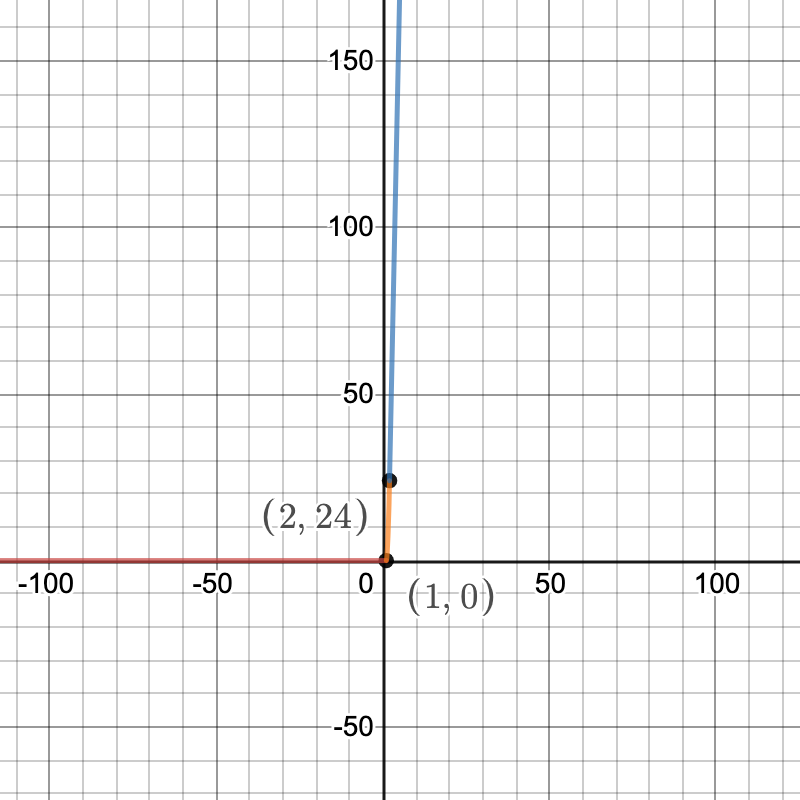
\includegraphics[width=7cm, height=7cm]{3a1.png}
            \captionof{figure}{Illustration of $M$-smooth} 
            }
            As is shown in Figure 1, it's easy to
            find that it's convex.

            \item strong convexity proof\\
            \indent the corresponding function $g(x)$ is,
            $$ g(x)=\left\{
                \begin{array}{lcl}
                24x^2       &      & {x      <      1}\\
                48x-24    &      & {1 \leq x \leq 2}\\
                24x^{2}-48x+72     &      & {x \geq 2}
                \end{array} \right. 
            $$
            {\centering
            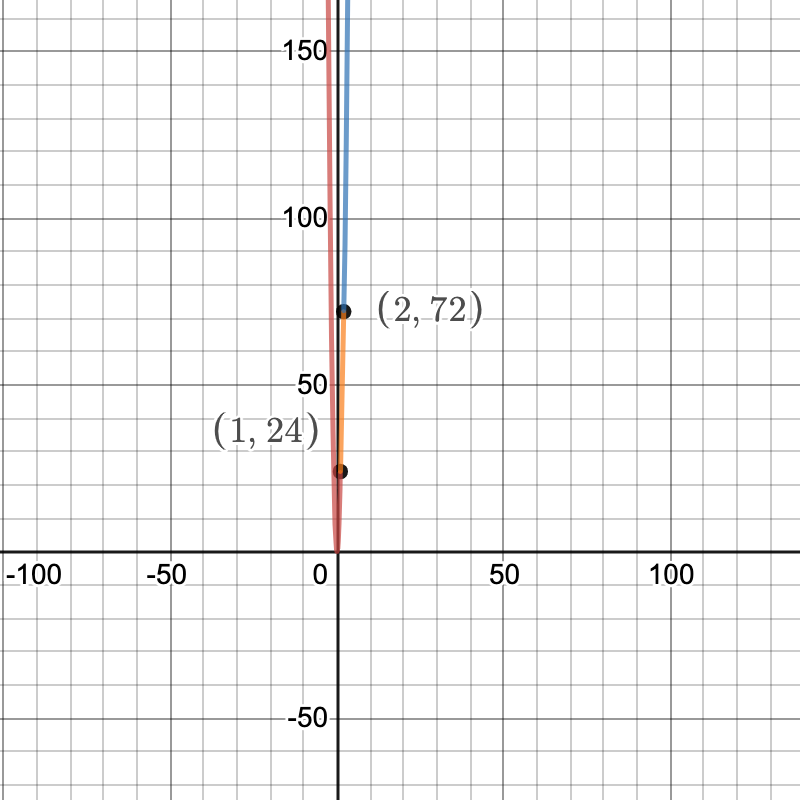
\includegraphics[width=7cm, height=7cm]{3a2.png}
            \captionof{figure}{Illustration of strong convexity} 
            }
            As is shown in Figure 2, it' easy to show it's convex.
        \end{itemize}

        \subsection{(b)}
        {\centering
        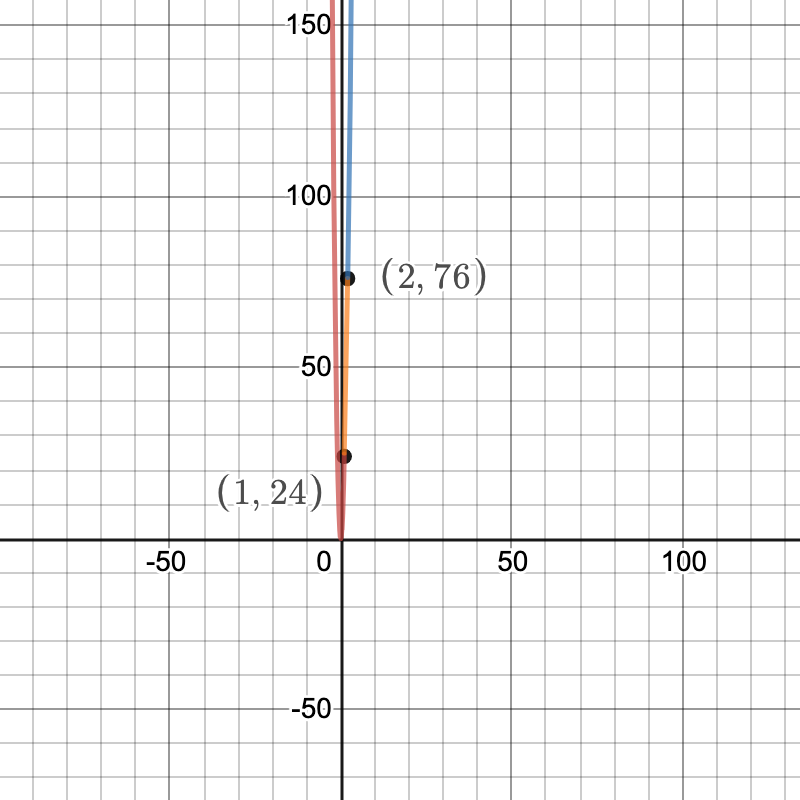
\includegraphics[width=7cm, height=7cm]{3b.png}
        \captionof{figure}{Illustration of global optimizer} 
        }
        As is shown in Figure 3, the global optimizer of 
        $f$ is $x^{\star}=0$\\

        \subsection{(c)}
        {\centering
        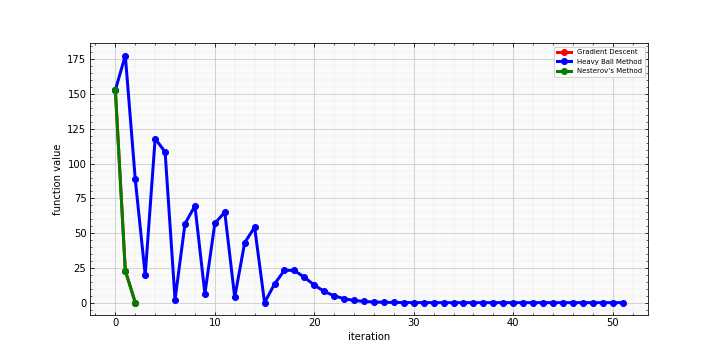
\includegraphics[width=14cm, height=7cm]{3c.png}
        \captionof{figure}{Illustration of global optimizer} 
        }
        Note that gradient descent and Nesterov's method has 
        the same plot.

        \subsection{(d)}
        {\centering
        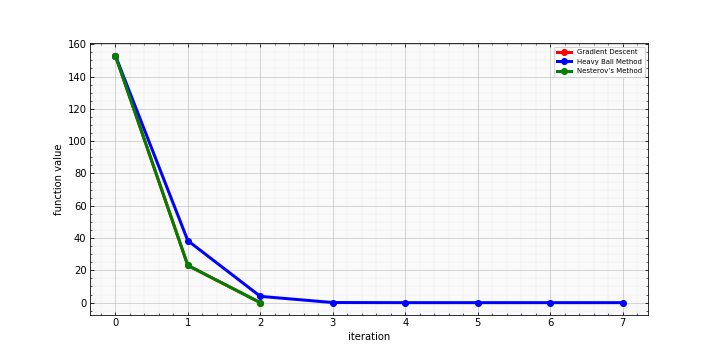
\includegraphics[width=14cm, height=7cm]{3d.png}
        \captionof{figure}{Illustration of global optimizer} 
        }
        Note that gradient descent and Nesterov's method has 
        the same plot.\\
        \indent For gradient descent, the best $\alpha$ is \textbf{1/50},
        the total iteration is \textbf{2}.
        For Heavy Ball Method, the best $\alpha$ is \textbf{0.017},
        the total iteration is \textbf{7}.
        For Nesterov's Method, the best $\alpha$ is \textbf{1/50},
        the total iteration is \textbf{2}.

    \end{framed}

    %%%%%%%%%%%%%%%%%%%%%%%%%%%%%%%%%%%%%%   Q4   %%%%%%%%%%%%%%%%%%%%%%%%%%%%%%%%%%%%%%%%%
    \begin{framed}
        \section{[Q4]}
        \subsection{(a)}
        Since $f$ is $M$-smooth, we can have,
        $$
        f(x_{k} + \alpha d_{k}) \leq f(x_{k}) + \langle \alpha d_{k},
        \nabla f(x_{k}) \rangle + \frac{M \alpha^{2}}{2} \lVert
        d_{k} \rVert_{2}^{2}
        $$
        \indent From given condition,
        $$
        \frac{M\alpha}{2} \lVert d_{k} \rVert_{2}^{2} \leq (c_{1}-1)
        \langle d_{k}, \nabla f(x_{k}) \rangle
        $$
        \indent we can have,
        $$
        f(x_{k}+\alpha d_{k}) \leq f(x_{k}) + \alpha \langle 
        d_{k}, \nabla f(x_{k})\rangle + \alpha(c_{1}-1) \langle 
        d_{k}, \nabla f(x_{k})\rangle
        $$
        \indent where we can simplify the right part as follows,
        $$
        f(x_{k}) + \alpha \langle 
        d_{k}, \nabla f(x_{k})\rangle + \alpha(c_{1}-1) \langle 
        d_{k}, \nabla f(x_{k})\rangle = f(x_{k}) + \alpha c_{1}
        \langle d_{k}, \nabla f(x_{k}) \rangle
        $$
        \indent Hence, we have
        $$
        f(x_{k}+\alpha d_{k}) \leq f(x_{k}) + \alpha c_{1}
        \langle d_{k}, \nabla f(x_{k}) \rangle
        $$

        \subsection{(b)}
        We can have,
        $$
            \alpha_{k} = \overline{\alpha} * \rho^{k} = \rho^{k}
        $$
        \indent since armijo condition tells us,
        \begin{align}
            \alpha_{k} &\leq 2(c_{1}-1)\frac{\langle d_{k},\nabla 
            f(x_{k}) \rangle}{M \lVert d_{k} \rVert_{2}^{2}} \\
            &\leq \frac{2(1-c_{1})}{M}
        \end{align}
        \indent where (1) to (2) follows $d_{k} = \nabla f(x_{k})$.\\
        \indent Hence, we can have
        $$
        \rho^{k} \leq \frac{2(1-c_{1})}{M}
        $$
        \indent And the number of backtracking iterations is 
        upper bouned by
        $$
        k \leq \log_{\rho}\frac{2}{M}(1-c_{1})
        $$
    \end{framed}

    %%%%%%%%%%%%%%%%%%%%%%%%%%%%%%%%%%%%%%   Q5   %%%%%%%%%%%%%%%%%%%%%%%%%%%%%%%%%%%%%%%%%
    \begin{framed}
        \section{[Q5]}
        \subsection{(a)}
        Yes, it's unique.

        \subsection{(b)}
        if $x_{0}$ is a minimizer of $f$, then it satisfies,
        $$
        f(x) \geq f(x_{0}), \quad\text{for all } x \in \text{dom} f
        $$
        \indent Now consider the second function, apprently, $x_{0}$
        is the minimizer of $\frac{\delta}{2} \lVert x-x_{0} \rVert_{2}^{2}$.\\
        \indent Hence, $x_{0}$ is the minimizer of $f_{\delta}{(x)}$, namely,
        $x_{\delta}^{\star} = x_{0}$.

        \subsection{(c)}
        By definition, we have,
        $$
        f_{\delta}(x_{\delta}^{\star}) \leq f_{\delta}(x)
        $$
        \indent for all $x \neq x_{\delta}^{\star}$ (including $x=x^{\star}$).\\
        \indent Hence we can have,
        \begin{align}
            f(x_{\delta}^{\star}) + \frac{\delta}{2} \lVert x_{\delta}^{\star}
             -x_{0} \rVert_{2}^{2} &\leq f(x^{\star}) + \frac{\delta}{2} 
             \lVert x^{\star}-x_{0} \rVert_{2}^{2}\\
            f(x_{\delta}^{\star}) &\leq f(x^{\star}) + \frac{\delta}{2} 
            \lVert x^{\star}-x_{0} \rVert_{2}^{2}
        \end{align}
        \indent where, (9) to (10) equality holds when $x_{\delta}^{\star}=x_{0}$.

        \subsection{(d)}
        \begin{itemize}
            \item $M_{\delta}$-smooth:\\
            Let's denote $g(x) = \frac{M_{\delta}}{2} \lVert x \rVert_{2}^{2} - f_{\delta}(x)$.
            we can have,
            \begin{align}
                \nabla^{2} g(x) &\geq 0\\
                M_{\delta} - \nabla^{2} f(x) - \delta &\geq 0\\
                \nabla^{2} f(x) &\leq M_{\delta} - \delta
            \end{align}
            \indent Since, $f(x)$ is convex, we have 
            $$
            \nabla^{2} f(x) \leq M \boldsymbol{I}
            $$
            Hence, we can conclude from that,
            $$
            M_{\delta} = M + \delta
            $$

            \item Strongly convex ($m_{\delta}$):\\
            Let's denote $h(x) = f_{\delta}(x) - \frac{m}{2}\lVert x \rVert_{2}^{2}$, we can have,
            \begin{align}
                \nabla^{2} h(x) &\geq 0 \\
                \nabla^{2} f(x) + \delta - m_{\delta} &\geq 0\\
                \nabla^{2} f(x) &\geq -\delta + m_{\delta}
            \end{align}
            \indent Since $f(x)$ is convex, we have $\nabla^{2}f(x)
            \geq 0$, hence, we can get,
            $$
            m_{\delta} = \delta
            $$
        \end{itemize}
    \end{framed}
    
    %%%%%%%%%%%%%%%%%%%%%%%%%%%%%%%%%%%%%%   Q6   %%%%%%%%%%%%%%%%%%%%%%%%%%%%%%%%%%%%%%%%%
    \begin{framed}
        \section{[Q6]}
        \subsection{(a)}
        the update rule is:
        $$
        p_{k+1}^{(n)} = p_{k}^{(n)} - \alpha_{k} * 4
        \sum\limits_{m\in N_{n}} (\lVert p^{(n)}-p^{(m)} \rVert_{2}^{2}-\Delta^{2})
        (p^{(n)}-p^{(m)})
        $$

        \subsection{(b)}
        {\centering
        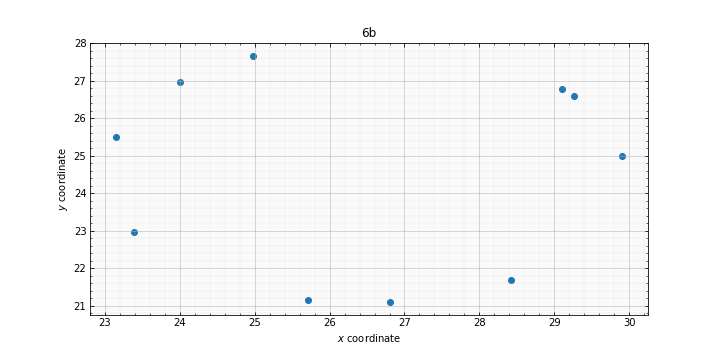
\includegraphics[width=14cm, height=7cm]{6b.png}
        \captionof{figure}{Illustration of global optimizer} 
        }
        I set $\alpha$ as \textbf{2e-5} and tolerance as
        \textbf{1e-5}, and the iteration
         is \textbf{6294}.

        \subsection{(c)}
        {\centering
        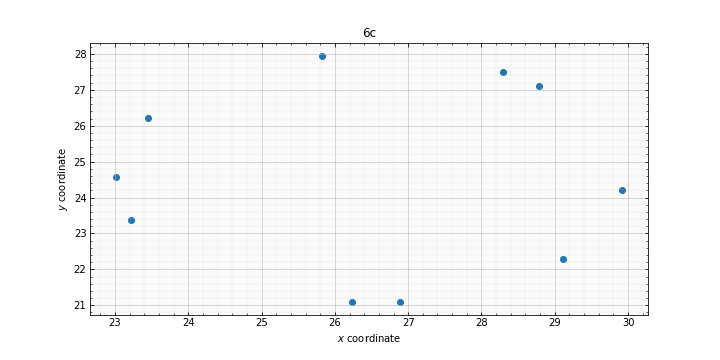
\includegraphics[width=14cm, height=7cm]{6c.png}
        \captionof{figure}{Illustration of global optimizer} 
        }
        I set $\alpha$ as \textbf{1e-5} and tolerance as 
        \textbf{1e-5}, and the iteration is \textbf{4179}.
        And the update rule is:
        $$
        p_{k+1}^{(n)} = p_{k}^{(n)} - \alpha_{k} * 4
        \sum\limits_{m\in N_{n}} (\lVert p^{(n)}-p^{(m)} \rVert_{2}^{2}-\Delta^{2})
        (p^{(n)}-p^{(m)})
        $$

        \subsection{(d)}
        $$
        \nabla^{2} f(p^{(n)}) = 4 \sum\limits_{m\in N_{n}} \left[ (\lVert
         p_{k}^{(n)}-p_{k}^{m} \rVert_{2}^{2} - \Delta^{2}) \boldsymbol{I}
         + 2(p_{k}^{(n)}-p_{k}^{(m)})(p_{k}^{(n)}-p_{k}^{(m)})^{T} \right]
        $$
        \indent Benefits: it will converge in far less iterations.\\
        \indent Drawbacks: it requires too much computation resouces to get hessian matrix.
    \end{framed}

    %%%%%%%%%%%%%%%%%%%%%%%%%%%%%%%%%%%%%%   Q7   %%%%%%%%%%%%%%%%%%%%%%%%%%%%%%%%%%%%%%%%%
    \begin{framed}
        \section{[Q7]}
        \subsection{(a)}
        Let's denote $f(\boldsymbol{x})$ as the object function, and we can get,
        $$
        \nabla f(\boldsymbol{x}) = (\lambda \boldsymbol{D} + \boldsymbol{I}) \boldsymbol{x} - \boldsymbol{y}
        $$
        \indent where, $\boldsymbol{I}$ is a $\mathbb{R}^{N * N}$ identity matrix.

        \subsection{(b)}
        $$
        \nabla^{2} f(\boldsymbol{x}) = \lambda \boldsymbol{D} + \boldsymbol{I}
        $$

        \subsection{(c)}
        \begin{align}
            \boldsymbol{x}_{k+1} &= \boldsymbol{x}_{k} - (\nabla^{2} f(\boldsymbol{x}_{k}))^{-1} \nabla f(\boldsymbol{x}_{k}) \\
            \boldsymbol{x}_{k+1} &= \boldsymbol{x}_{k} - (\lambda \boldsymbol{D} + \boldsymbol{I})^{-1} ((\lambda \boldsymbol{D} + \boldsymbol{I}) \boldsymbol{x}_{k}-\boldsymbol{y})\\
            \boldsymbol{x}_{k+1} &= \boldsymbol{x}_{k} - \boldsymbol{x}_{k} + (\lambda \boldsymbol{D} + \boldsymbol{I})^{-1} \boldsymbol{y}\\
            \boldsymbol{x}_{k+1} &= (\lambda \boldsymbol{D} + \boldsymbol{I})^{-1} \boldsymbol{y}
        \end{align}

        \subsection{(d)}
        Yes, it's a scalable solution to this problem when $N$ is very large. Because hessian matrix is a sparse matrix. When computing the inverse matrix, it's very fast.
    \end{framed}

    %%%%%%%%%%%%%%%%%%%%%%%%%%%%%%%%%%%%%%   Q8   %%%%%%%%%%%%%%%%%%%%%%%%%%%%%%%%%%%%%%%%%
    \begin{framed}
        \section{[Q8]}
        Note that the backtracking strategy here I used didn't always
        take $\alpha$ as $1.0$. Instead, it takes previous best $\alpha$
        as input and iterates again. The main reason I used this is Because
        i think it's more engineering. 
        \subsection{(a)}
        Here I set the minimum gradient tolerance as \textbf{1e-3}. And I think the best parameters
         of $c$ and $\rho$ are \textbf{0.1} and \textbf{0.2}. \textbf{962} 
         gradient steps are required when using line search method. By the combined
          backtracking searches, total number of iterations is \textbf{965}. Compared 
          with bisection which brings total iterations to 5120, backtracking 
          method is a more faster way to converge.

        \subsection{(b)}
        If we set $\alpha \approx 0.001$ and $\beta_{k} \approx 0.95$, it converge at iteration
        \textbf{383}. In best case, I set $\alpha$ as \textbf{0.001} and $\beta$ as \textbf{0.9}. 
        And the total iterations are \textbf{210}. From my persepctive, when using backtracking 
        to adjust $\alpha$ at each iteration(where $\beta$ is fixed as \textbf{0.9}), total 
        iterations are \textbf{210}. Combined backtracking, total iteration is \textbf{213}.

        \subsection{(c)}
        When setting $\alpha \approx 0.001$, the total iteration is \textbf{212}. When using
         backtracking, here i set the initial $\alpha$ as \textbf{0.5}, and the total 
         iteration is \textbf{162}. Combined with backtracking, total iteration is
         \textbf{166}.

        \subsection{(d)}
        When using backtracking, the total iteration is \textbf{6}.
        
        \subsection{(e)}
        When using backtracking, the total iteration is \textbf{12}. 
    \end{framed}

    %%%%%%%%%%%%%%% Appendix %%%%%%%%%%%%%%
    \section{Appendix}
    All the code can be found in my personal Github: \textbf{github.com/masqueraderx}
    \subsection{[Q3 code]}
        \begin{python}
import numpy as np
from matplotlib import pyplot as plt
# Define function and Gradient
def func(x):
    if x < 1:
        return 25*x**2
    elif 1<= x <= 2:
        return x**2 + 48*x - 24
    else:
        return 25*x**2 - 48*x + 72
    
def gradient(x):
    if x < 1:
        return 50*x
    elif 1<= x <= 2:
        return 2*x + 48
    else:
        return 50*x - 48

# gradient descent
alpha = 1 / 50
x=3
k=0
iterations_GD = [0]
values_GD = [func(x)]
while abs(gradient(x)) > 1e-3:
    dk = gradient(x)
    x = x - alpha * dk
    k += 1
    values_GD.append(func(x))
    iterations_GD.append(k)
    print('{}th iteration: gradient is {}, x is {}'.format(k, dk, x))

# heavy ball method
alpha = 0.017 #0.017
beta = 0.007 #0.007
x = [3,3]
k=1
iterations_HBM = [0]
values_HBM = [func(x[k])]
while abs(gradient(x[k])) > 1e-3:
    dk = gradient(x[k])
    x.append(x[k] - alpha * dk + beta * (x[k] - x[k-1]))
    k += 1
    iterations_HBM.append(k-1)
    values_HBM.append(func(x[k]))
    print('{}th iteration: gradient is {}, x is {}'.format(k-1, dk, x[k]))

# Nesterov's method
alpha = 1 / 50
x = [3,3]
k=1
iterations_NM = [0]
values_NM = [func(x[k])]
while abs(gradient(x[k])) > 1e-3:
    beta = (k-1)/(k+2)
    pk = beta*(x[k]-x[k-1])
    dk = gradient(x[k] + pk)
    x.append(x[k] + pk - alpha * dk)
    k += 1
    iterations_NM.append(k-1)
    values_NM.append(func(x[k]))
    print('{}th iteration: gradient is {}, x is {}'.format(k-1, gradient(x[k]), x[k]))

# Draw plot for three methods    
fid = plt.figure(figsize=(10,5))

Axes = plt.subplot(1,1,1)
Axes.axes.tick_params(which='both',direction='in',top=True, right=True)
plt.minorticks_on()
Axes.set_facecolor((0,0,0,0.02))

plt.plot(iterations_NM, values_NM, 'k-o', linewidth=3, color = 'r', label='Gradient Descent')
plt.plot(iterations_HBM, values_HBM, 'b-o', linewidth=3, label = 'Heavy Ball Method')
plt.plot(iterations_NM, values_NM, 'k-o', linewidth=3, color='g', label='Nesterov's Method')
plt.grid(True,which='major',linewidth=0.5)
plt.grid(True,which='minor',linewidth=0.1)
plt.xlabel("iteration")
plt.ylabel("function value")
plt.legend(loc='upper right',fontsize='x-small')
plt.savefig('/Users/gexueren/Desktop/6270/assignment/hw04/hw04/3d.png') 
        \end{python}
        
   
    \subsection{[Q6 code]}
        \begin{python} 
import numpy as np
from matplotlib import pyplot as plt
np.random.seed(2021)
p = np.random.uniform(0,50,[2,10])

#calculate gradient
def gradient(p, n, delta):
    d = np.zeros(2)
    for m in range(p.shape[1]):
        if m == n:
            continue
        else:
            d += np.multiply((np.linalg.norm(p[:,n]-p[:,m]))**2 - delta**2, p[:,n]-p[:,m])
    return d

#GD
def gradient_descent(p, alpha, maxiter, threshold):
    d = np.ones((2,10))
    k = 0
    while (k < maxiter) and (np.linalg.norm(d) > threshold):
        
        for i in range(p.shape[1]):
            d[:, i] = - gradient(p, i, 6)
        p = p + 4 * alpha * d
        k += 1
    print('final gradient is {}'.format(d[-1]))
    return p, k

# show results
points, iterations = gradient_descent(p, 2e-5, 10000, 1e-5)
print('points and total iteration is {} and {}'.format(points, iterations))
fid = plt.figure(figsize=(10,5))
Axes = plt.subplot(1,1,1)
Axes.axes.tick_params(which='both',direction='in',top=True, right=True)
plt.minorticks_on()
Axes.set_facecolor((0,0,0,0.02))
plt.scatter(points[0], points[1], label = 'points')
plt.grid(True,which='major',linewidth=0.5)
plt.grid(True,which='minor',linewidth=0.1)
plt.xlabel("$x$ coordinate")
plt.ylabel("$y$ coordinate")
# plt.legend(loc='upper right',fontsize='x-small')
plt.title('6b')
plt.savefig('/Users/gexueren/Desktop/6270/assignment/hw04/hw04/6b.png')

# Nesterov's method
def nesterov(p, alpha, maxiter, threshold):
    d = np.ones((2,10))
    k = 0
    pre_p = p
    pk = 0
    while (k < maxiter) and (np.linalg.norm(d) > threshold):
        beta = (k - 1) / (k + 2)
        for i in range(p.shape[1]):
            d[:, i] = - gradient(p + pk, i, 6)
        p = p + 4 * alpha * d + pk 
        pk = beta * (p - pre_p)
        k += 1
        pre_p = p
    print('final gradient is {}'.format(d[-1]))
    return p, k

points, iterations = nesterov(p, 1e-5, 10000, 1e-5)
print('points and total iteration is {} and {}'.format(points, iterations))
fid = plt.figure(figsize=(10,5))
Axes = plt.subplot(1,1,1)
Axes.axes.tick_params(which='both',direction='in',top=True, right=True)
plt.minorticks_on()
Axes.set_facecolor((0,0,0,0.02))
plt.scatter(points[0], points[1], label = 'points')
plt.grid(True,which='major',linewidth=0.5)
plt.grid(True,which='minor',linewidth=0.1)
plt.xlabel("$x$ coordinate")
plt.ylabel("$y$ coordinate")
# plt.legend(loc='upper right',fontsize='x-small')
plt.title('6c')
plt.savefig('/Users/gexueren/Desktop/6270/assignment/hw04/hw04/6c.png')
        \end{python}
    
    \subsection{[Q8 code]}
        \begin{python} 
import numpy as np
from sklearn import datasets
import math
import time
# the logistic function
def logistic_func(theta, x):
    t = x.T @ theta
    g = np.zeros(t.shape)
    # split into positive and negative to improve stability
    g[t>=0.0] = 1.0 / (1.0 + np.exp(-t[t>=0.0])) 
    g[t<0.0] = np.exp(t[t<0.0]) / (np.exp(t[t<0.0])+1.0)
    return g

# function to compute output of LR classifier
def lr_predict(theta,x):
    # form Xtilde for prediction
    x = np.vstack((x.T , np.ones(x.shape[0])))
    return logistic_func(theta,x)

# function to evaluate objective function (-f)
def f_eval(theta, x, y):
    t = x.T @ theta
    return -np.vdot(t,y) + np.sum(np.log(1+np.exp(t)))

# function to compute the gradient of -f
def grad(theta, x, y):
    g = logistic_func(theta,x)
    return -(x @ (y-g))

def hessian(theta, x):
    g = logistic_func(theta, x)
    n = g.shape[0]
    return np.dot(np.dot(np.dot(x, np.diag(g.reshape(n))), np.diag(1-g.reshape(n))), x.T)
    
    
# gradient descent
# returns theta and number of iterations
def gradDesc(x, y, alpha, c, rho, delta, maxiter, backTracking=False):
    # Initialization
    theta = np.zeros(x.shape[0])
    d = -grad(theta, x, y) # 3*1
    k = 0
    inner = 0
    while (k < maxiter) and (np.linalg.norm(d) > delta):
        '''
        this is backtracking tragetegy, Or should I say: Strategy :)
        '''
        if backTracking:
            alpha, m = back_tracking(x, y, theta, d, alpha, c, rho)
        theta = theta + alpha * d
        d = -grad(theta, x, y)
        k = k + 1
        if backTracking:
            inner = inner + m
    total = k + inner
    return theta, k, total


# heavy ball method
# returns theta and number of iterations
def heavyBall(x, y, alpha, beta, c, rho, delta, maxiter, backTracking=False):
    # Initialization
    theta = [np.zeros(x.shape[0]), np.zeros(x.shape[0])]
    d = -grad(theta[-1], x, y) # 3*1
    k = 1
    inner = 0
    while (k < maxiter) and (np.linalg.norm(d) > delta):
        '''
        this is backtracking tragetegy, Or should I say: Strategy :)
        '''
        if backTracking:
            alpha, m = back_tracking(x, y, theta[-1], d, alpha, c, rho)      
        theta.append(theta[k] + alpha * d + beta * (theta[k] - theta[k-1]))
        d = -grad(theta[-1], x, y)
        k = k + 1
        if backTracking:
            inner = inner + m
    total = k + inner
    return theta[-1], k-1, total-1



# nesterov's method
# returns theta and number of iterations
def nesterov(x, y, alpha, c, rho, delta, maxiter, backTracking=False):
    # Initialization
    theta = [np.zeros(x.shape[0]), np.zeros(x.shape[0])]
    d = -grad(theta[-1], x, y) # 3*1
    k = 1
    p = 0
    inner = 0
    while (k < maxiter) and (np.linalg.norm(d) > delta):
        '''
        this is backtracking tragetegy, Or should I say: Strategy :)
        '''
        if backTracking:
            alpha, m = back_tracking(x, y, theta[-1], d, alpha, c, rho)
        theta.append(theta[k] + alpha * d + p)
        k = k + 1
        beta = (k - 1) / (k + 2)
        p = beta * (theta[-1] - theta[-2])
        d = -grad(theta[-1] + p, x, y)
        if backTracking:
            inner = inner + m
    total = k + inner
    return theta[-1], k-1, total-1



# newton's method
# returns theta and number of iterations
def newton(x, y, alpha, c, rho, delta, maxiter, backTracking=False):
    # Initialization
    theta = np.zeros(x.shape[0])
    d = np.linalg.inv(hessian(theta, x)) @ (-grad(theta, x, y)) # 3*1
    k = 0
    inner = 0
    while (k < maxiter) and (np.linalg.norm(d) > delta):
        '''
        this is backtracking tragetegy, Or should I say: Strategy :)
        '''
        if backTracking:
            alpha, m = back_tracking(x, y, theta, d, alpha, c, rho)
        theta = theta + alpha * d
        d = np.linalg.inv(hessian(theta, x)) @ (-grad(theta, x, y))
        k = k + 1
        if backTracking:
            inner = inner + m
    total = inner + k
    return theta, k, total

def bfgs(x, y, alpha, c, rho, delta, maxiter, backTracking=False):
    # Initialization    
    theta = np.zeros(x.shape[0])

    h=np.linalg.inv(hessian(theta,x))
    g=grad(theta, x, y)
    d = -h @ g  
    k = 0
    inner = 0
    while (k < maxiter) and (np.linalg.norm(d) > delta):
        theta0 = theta
        g0 = g
        if backTracking:
            alpha, m = back_tracking(x, y, theta, d, alpha, c, rho)
        theta = theta + alpha*d
        g = grad(theta, x, y)
        s = np.mat(theta-theta0).T
        r = np.mat(g-g0).T
        a = h @ r
        gama=s.T @ r
        h = h + np.array((gama+(r.T @ a))/gama**2)*np.array((s @ s.T)) - np.array((a @ s.T)/gama) - np.array((s @ a.T)/gama)
        d = -h @ g
        k = k + 1
        if backTracking:
            inner = inner + m
        total = inner + k
    return theta, k, total  


# back_tracking
# returns alpha
def back_tracking(x, y, theta, d, alpha, c, rho):
    
    '''
    Phi function, see notes
    '''
    def phi(alpha):
        return f_eval(theta + alpha * d, x, y)
    '''
    h function, see notes
    '''
    def h(alpha):
        return f_eval(theta, x, y) + c * alpha * (d.T @ d)
    '''
    backtracking
    '''
    m = 0
    while phi(alpha) > h(alpha):
        alpha = rho * alpha
        m += 1
    return alpha, m

# Generate dataset
np.random.seed(2020) # Set random seed so results are repeatable
x,y = datasets.make_blobs(n_samples=100,n_features=2,centers=2,cluster_std=6.0)

# Form Xtilde
x = np.vstack((x.T , np.ones(x.shape[0])) ) #3*100

# Gradient Descent
'''
x: np.array
y: np.array
alpha: float
c: float 1e-4 - 0.3
rho: float 0.1 - 0.8
delta: float
maxiter: int
backTracking: bool, default: False
'''
# theta_gd, num_iters, total = gradDesc(x, y, 0.5, 0.1, 0.2, 1e-3, 10000, False)
theta_gd, num_iters, total = gradDesc(x, y, 0.5, 0.1, 0.2, 1e-3, 10000, True)
print('Number of iterations required (Gradient Descent): {0}'.format(num_iters))
print('Number of iterations required (Gradient Descent Combined backtracking): {0}'.format(total))
print('Solution: [{0} {1} {2}]^T'.format(theta_gd[0], theta_gd[1], theta_gd[2]))

# Heavy Ball Method
'''
x: np.array
y: np.array
alpha: float
beta: float
c: float
rho: float
delta: float
maxiter: int
backTracking: bool, default: False
'''

# theta_hbm, num_iters = heavyBall(x, y, 0.001, 0.95, 0.1, 0.2, 1e-3, 10000, False)
# theta_hbm, num_iters = heavyBall(x, y, 0.001, 0.9, 0.1, 0.2, 1e-3, 10000, False)
theta_hbm, num_iters, total = heavyBall(x, y, 0.25, 0.9, 0.1, 0.2, 1e-3, 10000, True)
print('Number of iterations required (Heavy Ball Method): {0}'.format(num_iters))
print('Number of iterations required (Heavy Ball Method Combined backtracking): {0}'.format(total))
print('Solution: [{0} {1} {2}]^T'.format(theta_hbm[0], theta_hbm[1], theta_hbm[2]))

# Nesterov's method
'''
x: np.array
y: np.array
alpha: float
c: float
rho: float
delta: float
maxiter: int
backTracking: bool, default: False
'''


# theta_nm, num_iters, total = nesterov(x, y, 0.001, 0.1, 0.2, 1e-3, 10000, False)
theta_nm, num_iters, total = nesterov(x, y, 0.5, 0.1, 0.2, 1e-3, 10000, True)
print('Number of iterations required (Nesterov\'s Method): {0}'.format(num_iters))
print('Number of iterations required (Nesterov\'s Method Combined backtracking): {0}'.format(total))
print('Solution: [{0} {1} {2}]^T'.format(theta_nm[0], theta_nm[1], theta_nm[2]))

# Newton's method
'''
x: np.array
y: np.array
alpha: float
c: float
rho: float
delta: float
maxiter: int
backTracking: bool, default: False
'''
# theta_Nm, num_iters, total = newton(x, y, 1.0, 0.1, 0.2, 1e-3, 10000, False)
theta_Nm, num_iters, total = newton(x, y, 1.0, 0.1, 0.2, 1e-3, 10000, True)
print('Number of iterations required (Newton\'s method): {0}'.format(num_iters))
print('Number of iterations required (Newton\'s Method  Combined backtracking): {0}'.format(total))
print('Solution: [{0} {1} {2}]^T'.format(theta_Nm[0], theta_Nm[1], theta_Nm[2]))

# BFGS
'''
x: np.array
y: np.array
alpha: float
c: float
rho: float
delta: float
maxiter: int
backTracking: bool, default: False
'''

theta_bfgs, num_iters, total = bfgs(x, y, 1.0, 0.1, 0.2, 1e-3, 10000, True)
print('Number of iterations required (BFGS): {0}'.format(num_iters))
print('Number of iterations required (BFGS Combined backtracking): {0}'.format(total))
print('Solution: [{0} {1} {2}]^T'.format(theta_bfgs[0], theta_bfgs[1], theta_bfgs[2]))
        \end{python}
\end{document}